\documentclass[12pt, letterpaper]{report}
\usepackage[margin=1in]{geometry}
\usepackage[utf8]{inputenc}
\usepackage{graphicx}
\usepackage{float}
\usepackage{subfig}
\usepackage{array}
\usepackage{color, colortbl}
\graphicspath{ {./img/} }
\setlength\parindent{0pt}
\renewcommand{\thesection}{\Roman{section}.}
\renewcommand{\thesubsection}{\arabic{subsection}.}
\definecolor{null}{gray}{0.8}


\title{ECE1166 - Cache-Coherence Protocol Analysis}
\author{Zachary M. Mattis}


\begin{document}
	
\maketitle


\section{State-Transition Diagrams}

% 1
\subsection{MSI w/ BusUpgr}

\begin{figure}[H]
	\centering
	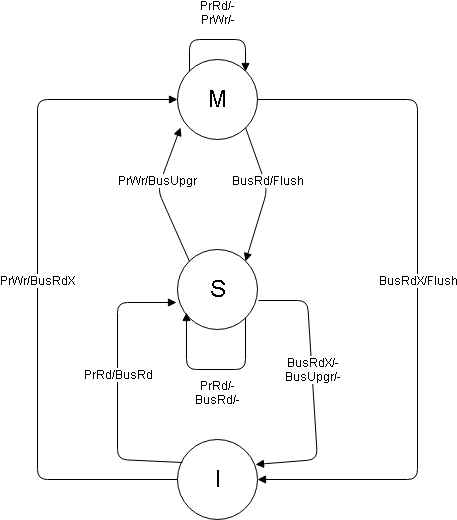
\includegraphics[width=0.4\columnwidth]{msi.png}
	\caption{MSI w/ BusUpgr}
\end{figure}


% 2
\subsection{MESI w/ no c2c sharing}

\begin{figure}[H]
	\centering
	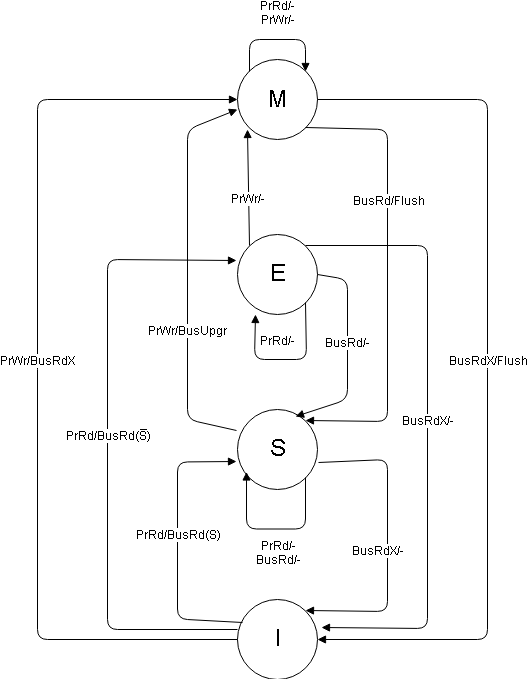
\includegraphics[width=0.4\columnwidth]{mesi_no_c2c.png}
	\caption{MESI w/ no c2c sharing}
\end{figure}


% 3
\subsection{MESI w/ M--I downgrade on BusRd}

\begin{figure}[H]
	\centering
	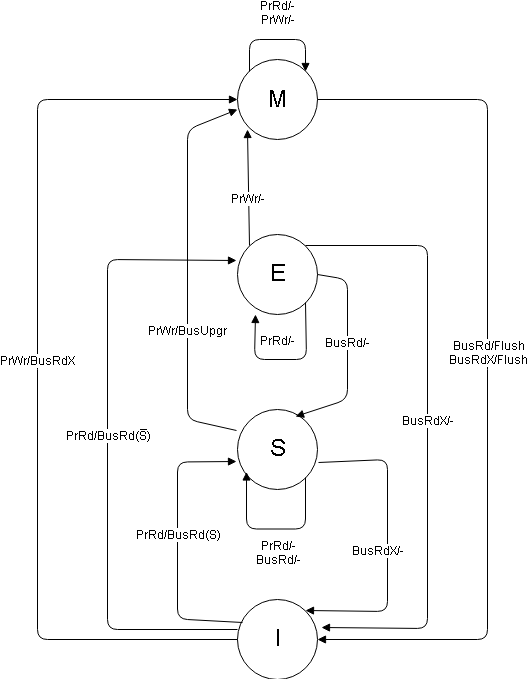
\includegraphics[width=0.4\columnwidth]{mesi_no_c2c_mi.png}
	\caption{MESI w/ M--I downgrade}
\end{figure}

Note: In the above diagram, cache controller in M state will transition to the I state on an observed BusRd, but will not assert its S line, allowing the reading cache controller to transition to E state via BusRd($\bar{S}$). It will still issue a flush in order to synchronize the modified block with lower memory.

% 4
\subsection{MESI w/ c2c sharing (M,E)}

\begin{figure}[H]
	\centering
	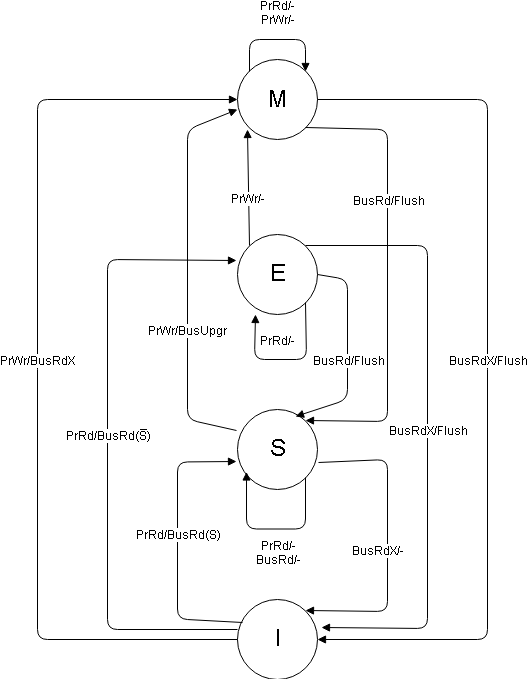
\includegraphics[width=0.4\columnwidth]{mesi_c2c.png}
	\caption{MESI w/ c2c sharing}
\end{figure}

Note: With cache-to-cache sharing enabled, the Flush commands issued by the M, E state cache controllers now imply direct sharing of the requested block.

% 5
\subsection{MESI w/ max c2c sharing via arbitration}

\begin{figure}[H]
	\centering
	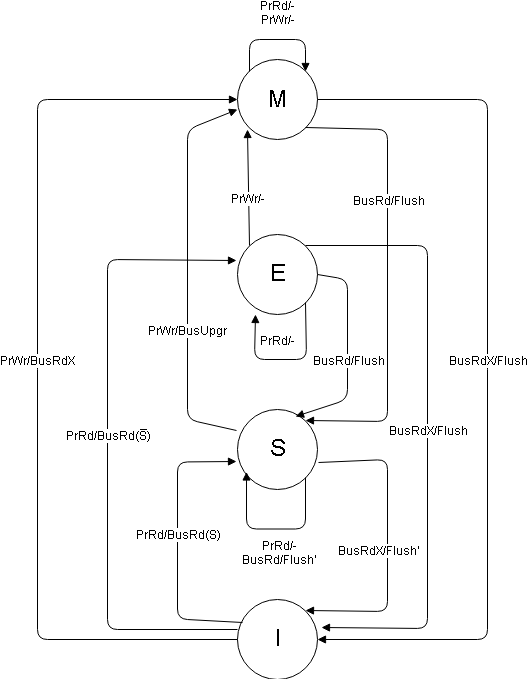
\includegraphics[width=0.4\columnwidth]{mesi_c2c_arb.png}
	\caption{MESI w/ arbitration c2c sharing}
\end{figure}

Note: Flush' implies cache blocks shared via peer arbitration to the requesting cache controller.

% 6
\subsection{MOESI}

\begin{figure}[H]
	\centering
	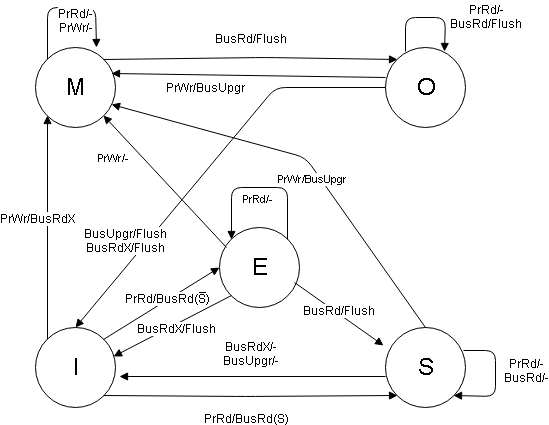
\includegraphics[width=0.6\columnwidth]{moesi.png}
	\caption{MOESI}
\end{figure}

% 7
\subsection{Dragon w/ max c2c sharing, no arbitration}

\begin{figure}[H]
	\centering
	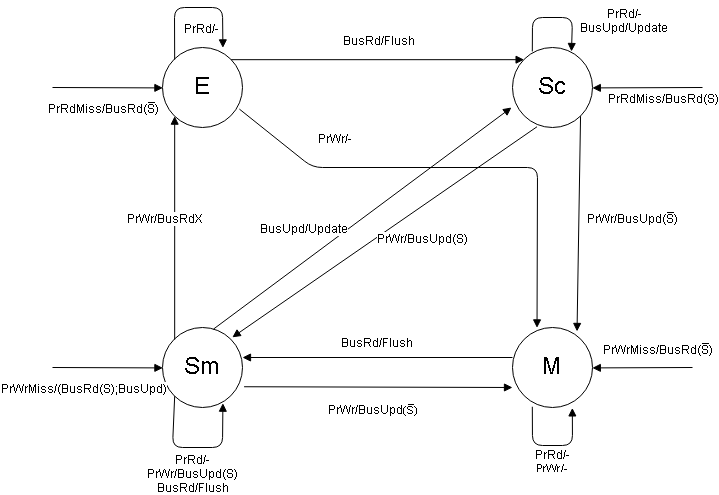
\includegraphics[width=0.6\columnwidth]{dragon.png}
	\caption{Dragon}
\end{figure}

\section{Memory Trace Campaigns}

% 1
\subsection{MSI w/ BusUpgr}

\begin{table}[H]
	\centering
	\begin{tabular}{ |c|r|c|c|c|l|r| }
		\hline
		\textbf{\#} & \textbf{Action} & \textbf{$P_1$} & \textbf{$P_{2}$} & \textbf{$P_3$} & \textbf{Bus} & \textbf{Cycles} \\
		\hline
		1 & r1 & S & - & - & BusRd & 200 \\
		\hline
		2 & w1 & M & - & - & BusUpgr & 40 \\
		\hline
		3 & r2 & S & S & - & BusRd/Flush & 200 \\
		\hline
		4 & w2 & I & M & - & BusUpgr & 40 \\
		\hline
		5 & r3 & I & S & S & BusRd/Flush & 200 \\
		\hline
		6 & w3 & I & I & M & BusUpgr & 40 \\
		\hline
		7 & r1 & S & I & S & BusRd/Flush & 200  \\
		\hline
		8 & w1 & M & I & I & BusUpgr & 40 \\
		\hline \hline \hline
		\cellcolor{null} & \cellcolor{null} & \cellcolor{null} & \cellcolor{null} & \cellcolor{null} & \textbf{Total} & \textbf{960} \\
		\hline
\end{tabular}
\caption{Access Sequence 1, Protocol 1\\MSI w/ BusUpgr}
\end{table}


\begin{table}[H]
	\centering
	\begin{tabular}{ |c|r|c|c|c|l|r| }
		\hline
		\textbf{\#} & \textbf{Action} & \textbf{$P_1$} & \textbf{$P_{2}$} & \textbf{$P_3$} & \textbf{Bus} & \textbf{Cycles} \\
		\hline
		1 & r1 & S & - & - & BusRd & 200 \\
		\hline
		2 & r2 & S & S & - & BusRd & 200 \\
		\hline
		3 & w1 & M & I & - & BusUpgr & 40 \\
		\hline
		4 & r3 & S & I & S & BusRd/Flush & 200 \\
		\hline
		5 & w2 & I & M & I & BusRdX & 200 \\
		\hline
		6 & r1 & S & S & I & BusRd/Flush & 200 \\
		\hline
		7 & w3 & I & I & M & BusRdX & 200 \\
		\hline
		8 & r2 & I & S & S & BusRd/Flush & 200 \\
		\hline
		9 & r3 & I & S & S & - & 1 \\
		\hline \hline \hline
		\cellcolor{null} & \cellcolor{null} & \cellcolor{null} & \cellcolor{null} & \cellcolor{null} & \textbf{Total} & \textbf{1441} \\
		\hline
	\end{tabular}
	\caption{Access Sequence 2, Protocol 1\\MSI w/ BusUpgr}
\end{table}


% 2
\subsection{MESI w/ no c2c sharing}

\begin{table}[H]
	\setlength{\extrarowheight}{.5ex}
	\centering
	\begin{tabular}{ |c|r|c|c|c|l|r| }
		\hline
		\textbf{\#} & \textbf{Action} & \textbf{$P_1$} & \textbf{$P_{2}$} & \textbf{$P_3$} & \textbf{Bus} & \textbf{Cycles} \\
		\hline
		1 & r1 & E & - & - & BusRd($\bar{S}$) & 200 \\
		\hline
		2 & w1 & M & - & - & - & 1 \\
		\hline
		3 & r2 & S & S & - & BusRd(S)/Flush & 200 \\
		\hline
		4 & w2 & I & M & - & BusUpgr & 40 \\
		\hline
		5 & r3 & I & S & S & BusRd(S)/Flush & 200 \\
		\hline
		6 & w3 & I & I & M & BusUpgr & 40 \\
		\hline
		7 & r1 & S & I & S & BusRd(S) & 200 \\
		\hline
		8 & w1 & M & I & I & BusUpgr & 40 \\
		\hline \hline \hline
		\cellcolor{null} & \cellcolor{null} & \cellcolor{null} & \cellcolor{null} & \cellcolor{null} & \textbf{Total} & \textbf{921} \\
		\hline
	\end{tabular}
	\caption{Access Sequence 1, Protocol 2\\MESI w/ no c2c sharing}
\end{table}


\begin{table}[H]
	\setlength{\extrarowheight}{.5ex}
	\centering
	\begin{tabular}{ |c|r|c|c|c|l|r| }
		\hline
		\textbf{\#} & \textbf{Action} & \textbf{$P_1$} & \textbf{$P_{2}$} & \textbf{$P_3$} & \textbf{Bus} & \textbf{Cycles} \\
		\hline
		1 & r1 & E & - & - & BusRd($\bar{S}$) & 200 \\
		\hline
		2 & r2 & S & S & - & BusRd(S) & 200 \\
		\hline
		3 & w1 & M & I & - & BusUpgr & 40 \\
		\hline
		4 & r3 & S & I & S & BusRd(S)/Flush & 200 \\
		\hline
		5 & w2 & I & M & I & BusRdX & 200 \\
		\hline
		6 & r1 & S & S & I & BusRd(S)/Flush & 200 \\
		\hline
		7 & w3 & I & I & M & BusRdX & 200 \\
		\hline
		8 & r2 & I & S & S & BusRd(S)/Flush & 200 \\
		\hline
		9 & r3 & I & S & S & - & 1 \\
		\hline \hline \hline
		\cellcolor{null} & \cellcolor{null} & \cellcolor{null} & \cellcolor{null} & \cellcolor{null} & \textbf{Total} & \textbf{1441} \\
		\hline
	\end{tabular}
	\caption{Access Sequence 2, Protocol 2\\MESI w/ no c2c sharing}
\end{table}


% 3
\subsection{MESI w/ M--I downgrade on BusRd}

\begin{table}[H]
	\setlength{\extrarowheight}{.5ex}
	\centering
	\begin{tabular}{ |c|r|c|c|c|l|r| }
		\hline
		\textbf{\#} & \textbf{Action} & \textbf{$P_1$} & \textbf{$P_{2}$} & \textbf{$P_3$} & \textbf{Bus} & \textbf{Cycles} \\
		\hline
		1 & r1 & E & - & - & BusRd($\bar{S}$) & 200 \\
		\hline
		2 & w1 & M & - & - & - & 1 \\
		\hline
		3 & r2 & I & E & - & BusRd($\bar{S}$)/Flush & 200 \\
		\hline
		4 & w2 & I & M & - & - & 1 \\
		\hline
		5 & r3 & I & I & E & BusRd($\bar{S}$)/Flush & 200 \\
		\hline
		6 & w3 & I & I & M & - & 1 \\
		\hline
		7 & r1 & E & I & I & BusRd($\bar{S}$)/Flush & 200 \\
		\hline
		8 & w1 & M & I & I & - & 1 \\
		\hline \hline \hline
		\cellcolor{null} & \cellcolor{null} & \cellcolor{null} & \cellcolor{null} & \cellcolor{null} & \textbf{Total} & \textbf{804} \\
		\hline
	\end{tabular}
	\caption{Access Sequence 1, Protocol 3\\MESI w/ M--I downgrade on BusRd}
\end{table}


\begin{table}[H]
	\setlength{\extrarowheight}{.5ex}
	\centering
	\begin{tabular}{ |c|r|c|c|c|l|r| }
		\hline
		\textbf{\#} & \textbf{Action} & \textbf{$P_1$} & \textbf{$P_{2}$} & \textbf{$P_3$} & \textbf{Bus} & \textbf{Cycles} \\
		\hline
		1 & r1 & E & - & - & BusRd($\bar{S}$) & 200 \\
		\hline
		2 & r2 & S & S & - & BusRd(S) & 200 \\
		\hline
		3 & w1 & M & I & - & BusUpgr & 40 \\
		\hline
		4 & r3 & I & I & E & BusRd($\bar{S}$)/Flush & 200 \\
		\hline
		5 & w2 & I & M & I & BusRdX & 200 \\
		\hline
		6 & r1 & E & I & I & BusRd($\bar{S}$)/Flush & 200 \\
		\hline
		7 & w3 & I & I & M & BusRdX & 200 \\
		\hline
		8 & r2 & I & E & I & BusRd($\bar{S}$)/Flush & 200 \\
		\hline
		9 & r3 & I & S & S & BusRd(S) & 200 \\
		\hline \hline \hline
		\cellcolor{null} & \cellcolor{null} & \cellcolor{null} & \cellcolor{null} & \cellcolor{null} & \textbf{Total} & \textbf{1640} \\
		\hline
	\end{tabular}
	\caption{Access Sequence 2, Protocol 3\\MESI w/ M--I downgrade on BusRd}
\end{table}



% 4
\subsection{MESI w/ c2c sharing (M,E)}

\begin{table}[H]
	\setlength{\extrarowheight}{.5ex}
	\centering
	\begin{tabular}{ |c|r|c|c|c|l|r| }
		\hline
		\textbf{\#} & \textbf{Action} & \textbf{$P_1$} & \textbf{$P_{2}$} & \textbf{$P_3$} & \textbf{Bus} & \textbf{Cycles} \\
		\hline
		1 & r1 & E & - & - & BusRd($\bar{S}$) & 200 \\
		\hline
		2 & w1 & M & - & - & - & 1 \\
		\hline
		3 & r2 & S & S & - & BusRd(S)/Flush & 80 \\
		\hline
		4 & w2 & I & M & - & BusUpgr & 40 \\
		\hline
		5 & r3 & I & S & S & BusRd(S)/Flush & 80 \\
		\hline
		6 & w3 & I & I & M & BusUpgr & 40 \\
		\hline
		7 & r1 & S & I & S & BusRd(S)/Flush & 80 \\
		\hline
		8 & w1 & M & I & I & BusUpgr & 40 \\
		\hline \hline \hline
		\cellcolor{null} & \cellcolor{null} & \cellcolor{null} & \cellcolor{null} & \cellcolor{null} & \textbf{Total} & \textbf{561} \\
		\hline
	\end{tabular}
	\caption{Access Sequence 1, Protocol 4\\MESI w/ c2c sharing (M,E)}
\end{table}


\begin{table}[H]
	\setlength{\extrarowheight}{.5ex}
	\centering
	\begin{tabular}{ |c|r|c|c|c|l|r| }
		\hline
		\textbf{\#} & \textbf{Action} & \textbf{$P_1$} & \textbf{$P_{2}$} & \textbf{$P_3$} & \textbf{Bus} & \textbf{Cycles} \\
		\hline
		1 & r1 & E & - & - & BusRd($\bar{S}$) & 200 \\
		\hline
		2 & r2 & S & S & - & BusRd(S)/Flush & 80 \\
		\hline
		3 & w1 & M & I & - & BusUpgr & 40 \\
		\hline
		4 & r3 & S & I & S & BusRd(S)/Flush & 80 \\
		\hline
		5 & w2 & I & M & I & BusRdX & 200 \\
		\hline
		6 & r1 & S & S & I & BusRd(S)/Flush & 80 \\
		\hline
		7 & w3 & I & I & M & BusRdX & 200 \\
		\hline
		8 & r2 & I & S & S & BusRd(S)/Flush & 80 \\
		\hline
		9 & r3 & I & S & S & - & 1 \\
		\hline \hline \hline
		\cellcolor{null} & \cellcolor{null} & \cellcolor{null} & \cellcolor{null} & \cellcolor{null} & \textbf{Total} & \textbf{961} \\
		\hline
	\end{tabular}
	\caption{Access Sequence 2, Protocol 4\\MESI w/ c2c sharing (M,E)}
\end{table}



% 5
\subsection{MESI w/ max c2c sharing via arbitration}

\begin{table}[H]
	\setlength{\extrarowheight}{.5ex}
	\centering
	\begin{tabular}{ |c|r|c|c|c|l|r| }
		\hline
		\textbf{\#} & \textbf{Action} & \textbf{$P_1$} & \textbf{$P_{2}$} & \textbf{$P_3$} & \textbf{Bus} & \textbf{Cycles} \\
		\hline
		1 & r1 & E & - & - & BusRd($\bar{S}$) & 200 \\
		\hline
		2 & w1 & M & - & - & - & 1 \\
		\hline
		3 & r2 & S & S & - & BusRd(S)/Flush & 80 \\
		\hline
		4 & w2 & I & M & - & BusUpgr & 40 \\
		\hline
		5 & r3 & I & S & S & BusRd(S)/Flush & 80 \\
		\hline
		6 & w3 & I & I & M & BusUpgr & 40 \\
		\hline
		7 & r1 & S & I & S & BusRd(S)/Flush & 80 \\
		\hline
		8 & w1 & M & I & I & BusUpgr & 40 \\
		\hline \hline \hline
		\cellcolor{null} & \cellcolor{null} & \cellcolor{null} & \cellcolor{null} & \cellcolor{null} & \textbf{Total} & \textbf{561} \\
		\hline
	\end{tabular}
	\caption{Access Sequence 1, Protocol 5\\MESI w/ max c2c sharing via arbitration}
\end{table}


\begin{table}[H]
	\setlength{\extrarowheight}{.5ex}
	\centering
	\begin{tabular}{ |c|r|c|c|c|l|r| }
		\hline
		\textbf{\#} & \textbf{Action} & \textbf{$P_1$} & \textbf{$P_{2}$} & \textbf{$P_3$} & \textbf{Bus} & \textbf{Cycles} \\
		\hline
		1 & r1 & E & - & - & BusRd($\bar{S}$) & 200 \\
		\hline
		2 & r2 & S & S & - & BusRd(S)/Flush & 80 \\
		\hline
		3 & w1 & M & I & - & BusUpgr & 40 \\
		\hline
		4 & r3 & S & I & S & BusRd(S)/Flush & 80 \\
		\hline
		5 & w2 & I & M & I & BusRdX/Flush' & 100 \\
		\hline
		6 & r1 & S & S & I & BusRd(S)/Flush & 80 \\
		\hline
		7 & w3 & I & I & M & BusRdX/Flush' & 100 \\
		\hline
		8 & r2 & I & S & S & BusRd(S)/Flush & 80 \\
		\hline
		9 & r3 & I & S & S & - & 1 \\
		\hline \hline \hline
		\cellcolor{null} & \cellcolor{null} & \cellcolor{null} & \cellcolor{null} & \cellcolor{null} & \textbf{Total} & \textbf{761} \\
		\hline
	\end{tabular}
	\caption{Access Sequence 2, Protocol 5\\MESI w/ max c2c sharing via arbitration}
\end{table}


% 6
\subsection{MOESI}

\begin{table}[H]
	\setlength{\extrarowheight}{.5ex}
	\centering
	\begin{tabular}{ |c|r|c|c|c|l|r| }
		\hline
		\textbf{\#} & \textbf{Action} & \textbf{$P_1$} & \textbf{$P_{2}$} & \textbf{$P_3$} & \textbf{Bus} & \textbf{Cycles} \\
		\hline
		1 & r1 & E & - & - & BusRd($\bar{S}$) & 200 \\
		\hline
		2 & w1 & M & - & - & - & 1 \\
		\hline
		3 & r2 & O & S & - & BusRd(S)/Flush & 80 \\
		\hline
		4 & w2 & I & M & - & BusUpgr & 40 \\
		\hline
		5 & r3 & I & O & S & BusRd(S)/Flush & 80 \\
		\hline
		6 & w3 & I & I & M & BusUpgr & 40 \\
		\hline
		7 & r1 & S & I & O & BusRd(S)/Flush & 80 \\
		\hline
		8 & w1 & M & I & I & BusUpgr & 40 \\
		\hline \hline \hline
		\cellcolor{null} & \cellcolor{null} & \cellcolor{null} & \cellcolor{null} & \cellcolor{null} & \textbf{Total} & \textbf{561} \\
		\hline
	\end{tabular}
	\caption{Access Sequence 1, Protocol 6\\MOESI}
\end{table}


\begin{table}[H]
	\setlength{\extrarowheight}{.5ex}
	\centering
	\begin{tabular}{ |c|r|c|c|c|l|r| }
		\hline
		\textbf{\#} & \textbf{Action} & \textbf{$P_1$} & \textbf{$P_{2}$} & \textbf{$P_3$} & \textbf{Bus} & \textbf{Cycles} \\
		\hline
		1 & r1 & E & - & - & BusRd($\bar{S}$) & 200 \\
		\hline
		2 & r2 & S & S & - & BusRd(S)/Flush & 80 \\
		\hline
		3 & w1 & M & I & - & BusUpgr & 40 \\
		\hline
		4 & r3 & O & I & S & BusRd(S)/Flush & 80 \\
		\hline
		5 & w2 & I & M & I & BusRdX/Flush & 80 \\
		\hline
		6 & r1 & S & O & I & BusRd(S)/Flush & 80 \\
		\hline
		7 & w3 & I & I & M & BusRdX/Flush & 80 \\
		\hline
		8 & r2 & I & S & O & BusRd(S)/Flush & 80 \\
		\hline
		9 & r3 & I & S & O & - & 1 \\
		\hline \hline \hline
		\cellcolor{null} & \cellcolor{null} & \cellcolor{null} & \cellcolor{null} & \cellcolor{null} & \textbf{Total} & \textbf{721} \\
		\hline
	\end{tabular}
	\caption{Access Sequence 2, Protocol 6\\MOESI}
\end{table}



% 7
\subsection{Dragon w/ max c2c sharing, no arbitration}

\begin{table}[H]
	\setlength{\extrarowheight}{.5ex}
	\centering
	\begin{tabular}{ |c|r|c|c|c|l|r| }
		\hline
		\textbf{\#} & \textbf{Action} & \textbf{$P_1$} & \textbf{$P_{2}$} & \textbf{$P_3$} & \textbf{Bus} & \textbf{Cycles} \\
		\hline
		1 & r1 & E & - & - & BusRd($\bar{S}$) & 200 \\
		\hline
		2 & w1 & M & - & - & - & 1 \\
		\hline
		3 & r2 & Sm & Sc & - & BusRd(S)/Flush & 80 \\
		\hline
		4 & w2 & Sc & Sm & - & BusUpd(S) & 40 \\
		\hline
		5 & r3 & Sc & Sm & Sc & BusRd(S)/Flush & 80 \\
		\hline
		6 & w3 & Sc & Sc & Sm & BusUpd(S) & 40 \\
		\hline
		7 & r1 & Sc & Sc & Sm & - & 1 \\
		\hline
		8 & w1 & Sm & Sc & Sc & BusUpd(S) & 40 \\
		\hline \hline \hline
		\cellcolor{null} & \cellcolor{null} & \cellcolor{null} & \cellcolor{null} & \cellcolor{null} & \textbf{Total} & \textbf{482} \\
		\hline
	\end{tabular}
	\caption{Access Sequence 1, Protocol 7\\Dragon}
\end{table}


\begin{table}[H]
	\setlength{\extrarowheight}{.5ex}
	\centering
	\begin{tabular}{ |c|r|c|c|c|l|r| }
		\hline
		\textbf{\#} & \textbf{Action} & \textbf{$P_1$} & \textbf{$P_{2}$} & \textbf{$P_3$} & \textbf{Bus} & \textbf{Cycles} \\
		\hline
		1 & r1 & E & - & - & BusRd($\bar{S}$) & 200 \\
		\hline
		2 & r2 & Sc & Sc & - & BusRd(S)/Flush & 80 \\
		\hline
		3 & w1 & Sm & Sc & - & BusUpd(S) & 40 \\
		\hline
		4 & r3 & Sm & Sc & Sc & BusRd(S)/Flush & 80 \\
		\hline
		5 & w2 & Sc & Sm & Sc & BusUpd(S) & 40 \\
		\hline
		6 & r1 & Sc & Sm & Sc & - & 1 \\
		\hline
		7 & w3 & Sc & Sc & Sm & BusUpd(S) & 40 \\
		\hline
		8 & r2 & Sc & Sc & Sm & - & 1 \\
		\hline
		9 & r3 & Sc & Sc & Sm & - & 1 \\
		\hline \hline \hline
		\cellcolor{null} & \cellcolor{null} & \cellcolor{null} & \cellcolor{null} & \cellcolor{null} & \textbf{Total} & \textbf{483} \\
		\hline
	\end{tabular}
	\caption{Access Sequence 2, Protocol 7\\Dragon}
\end{table}

\section{Cache Coherence Analysis}

\begin{table}[H]
	\centering
	\begin{tabular}{ |l|r|r| }
		\hline
		\textbf{Protocol} & \textbf{Sequence 1} & \textbf{Sequence 2} \\
		\hline
		\textbf{MSI w/ BusUpgr} & 960 & 1441 \\
		\hline
		\textbf{MESI w/ no c2c sharing} & 921 & 1441 \\
		\hline
		\textbf{MESI w/ M--I downgrade} & 804 & 1640 \\
		\hline
		\textbf{MESI w/ c2c sharing} & 561 & 961 \\
		\hline
		\textbf{MESI w/ arbitration c2c sharing} & 561 & 761 \\
		\hline
		\textbf{MOESI} & 561 & 721 \\
		\hline
		\textbf{Dragon} & 482 & 483 \\
		\hline	
	\end{tabular}
	\caption{Cache Coherence Protocol Cycle Time}
\end{table}


Based on the memory access patterns for the above cache coherence protocols, Dragon appeared to be the most successfully. This is largely due to the small time that it takes to update the word of block in other cache controllers, which is only 40 cycles. This benefit can be seen as the invalidated blocks of other (invalidation) protocols must then get their blocks from other caches controllers (80 cycles) or from lower memory (200 cycles).
\\ \\
The benefits of cache-to-cache sharing can be observed on the MESI protocols, both with and without arbitration. These protocols illustrated much greater improvements in total cycle time compared to their non-c2c sharing counterparts.
\\ \\
One of the more interesting protocols was the M--I downgrade for MESI on BusRd. This protocol showed performance improvements with data migratory patterns where the data read was then immediately modified. This benefit is observed as the subsequent write to the data block does not have to issue a BusUpgr command to the other cache controller, as M blocks are automatically demoted to I state. This has great drawbacks, as illustrated by the second memory access pattern, providing the worst overall access time. This is largely due to the pattern not taking advantage of the exclusive state to write to data, especially when their is no cache-to-cache sharing enabled.
\\ \\
It is not surprising that as the complexity of the cache-coherence protocol increases, the performance of it also increases, leading to lower total cycle times.

\end{document}